\Subsubsubsection{Potencia}

Para la unidad de potencia se utilizarán paneles solares y una batería de gel de ciclo profundo conectados a la placa DFR0580, la cual se ocupa de cargar la batería. De esta se obtienen 4 salidas de tensión:
\begin{itemize}
	\item Dos salidas de 5 V y 2.5 A [USB].
	\item Una salida de 5 V y 5 A.
	\item Una salida de 12 V y 8 A.
\end{itemize}

Con estas salidas se alimentarán todos los módulos, a excepción del oscilador de potencia, ya que esta necesita una etapa DC-DC para así la cual eleva la tensión. Para ello se emplea una fuente switching de topología Boost.

\Subsubsubsection{Cargador}

El bloque del cargador de la UBM consiste en un receptor y un transmisor de potencia. La transmisión inalámbrica consta, por el lado del transmisor, de un oscilador de $915 \ MHz$, el cual está comandado por la R-Pi, y un amplificador de potencia alimentado por otra etapa DC-DC de 12 V a 15 V.

Por el lado del receptor, se encuentra el integrado P1110B, el cual estabiliza la energía para realizar la carga de la UBM.

\begin{figure}[H]
	\centering
	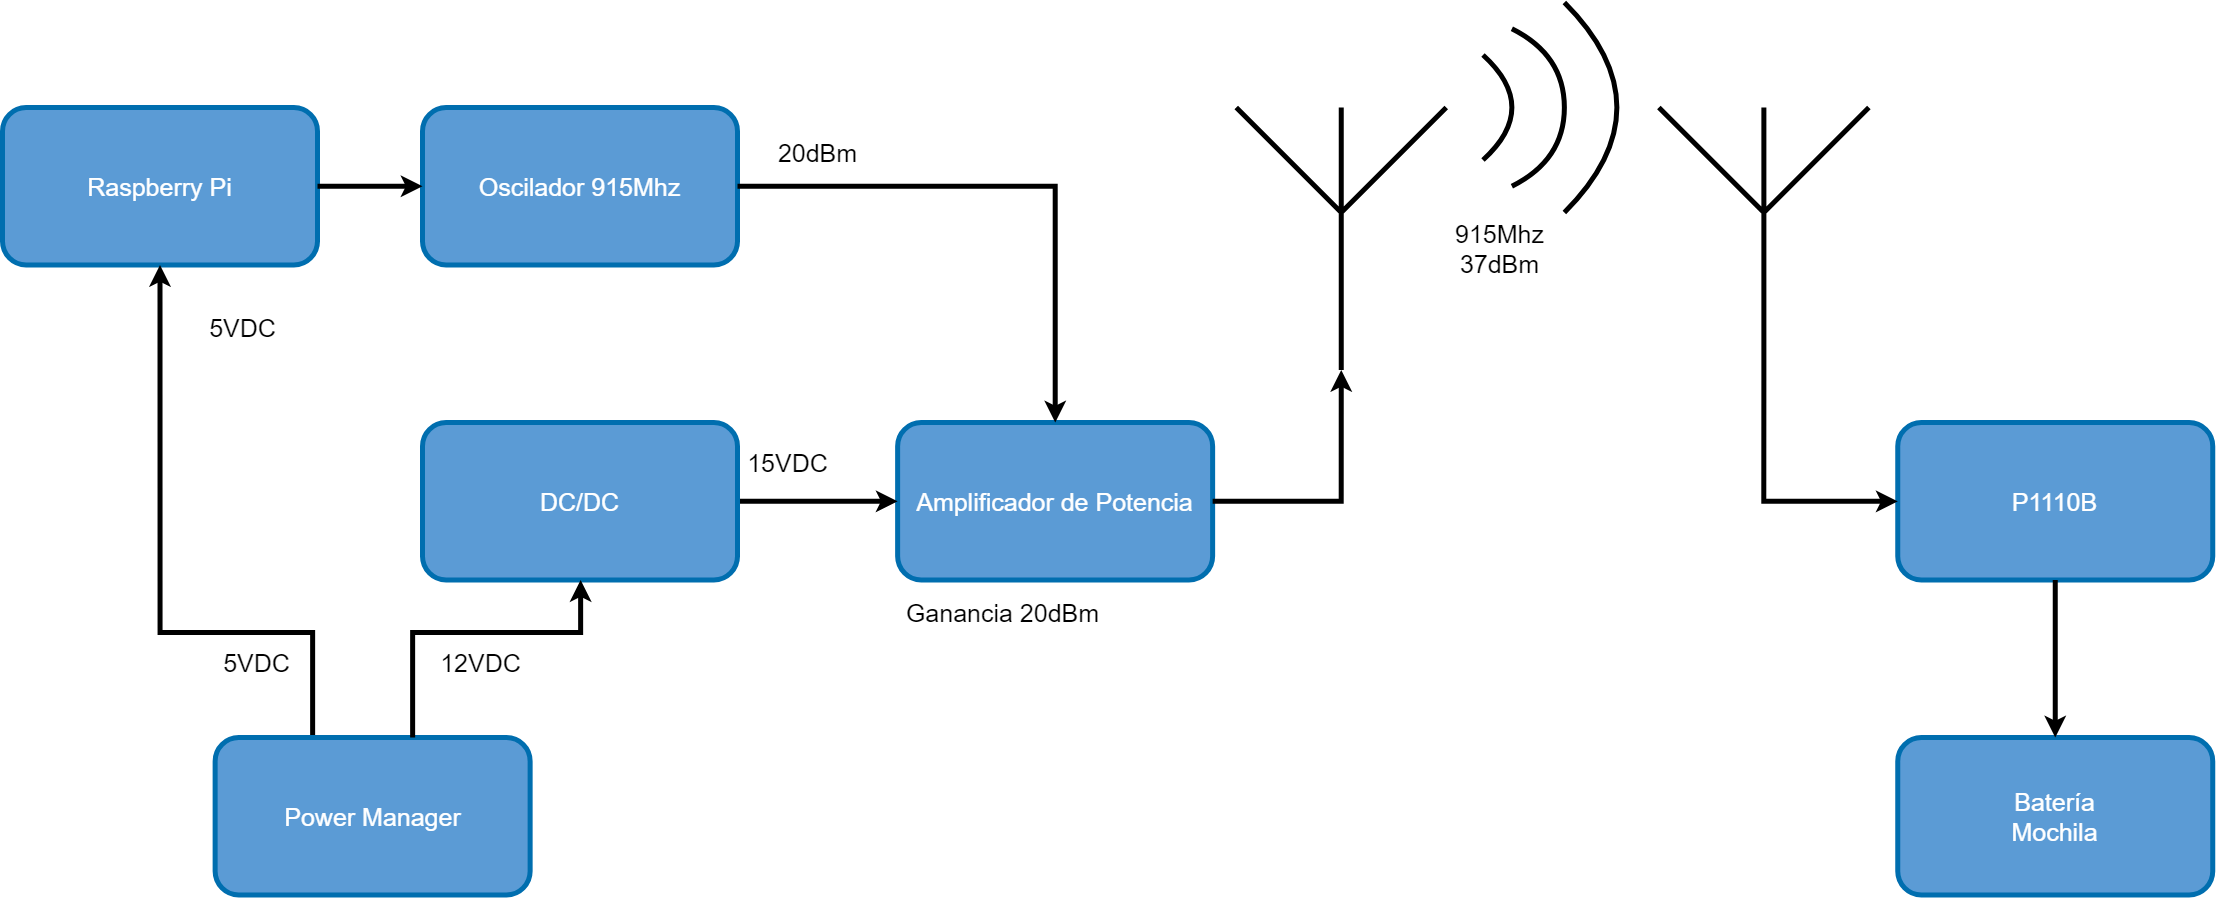
\includegraphics[width=0.9\linewidth]{ImagenesIngenieria de Detalle/EsquemaHardwareAntenas}	
	\caption{Diagrama en bloques cargador.}
	\label{fig:diagrama_hardware_antenas}
\end{figure}

\Subsubsubsection{Sensado}

En esta sección, ademas del conexionado de los sensores, se hace detalle en los pines de la R-Pi que serán utilizados.

\begin{figure}[H]
	\centering
	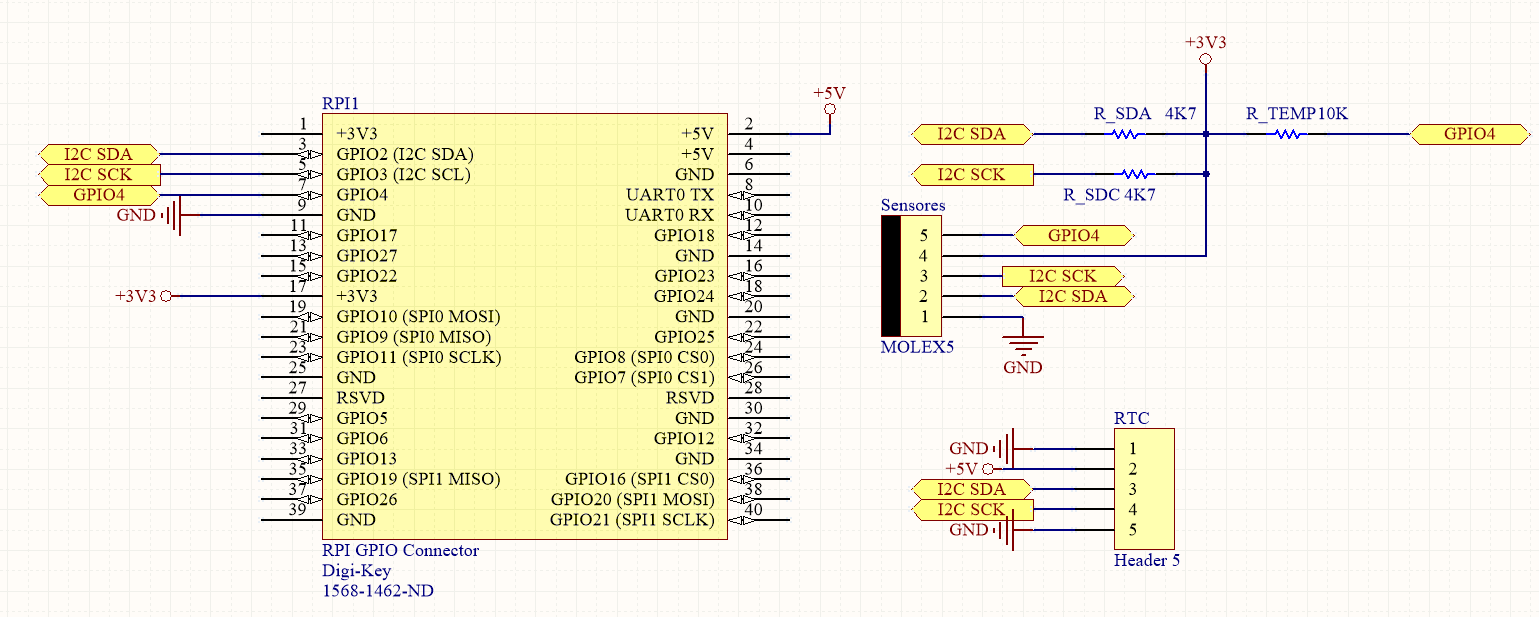
\includegraphics[width=0.9\linewidth]{ImagenesIngenieria de Detalle/Conexionado_rpi}		
	\caption{Conexionado Raspberry Pi.}
	\label{fig:conexionado_Rpi}
\end{figure}

El sensor de humedad y temperatura (DHT-22) se comunica de manera serial a través de un pin de GPIO. Para que esto sea posible, el sensor necesita alimentación de 3.3 V, tierra y el pin de GPIO por donde se realiza la comunicación, teniendo en cuenta que es necesario una resistencia de pull-up entre la linea de datos y 3.3 V.

El oscilador necesita de una señal de alimentación, tierra y su comunicación utilizá el protocolo UART. Por otro lado, la cámara simplemente se conecta al zócalo destinado para este propósito en la placa. Para el conexionado con el sensor de luminosidad y RTC se utilizará el protocolo de comunicación $I^2C$ en modo multi-slave.

Finalmente, se cuenta con un pin de GPIO el cual indicará el momento de prendido del cargador.

\begin{figure}[H]
	\centering
	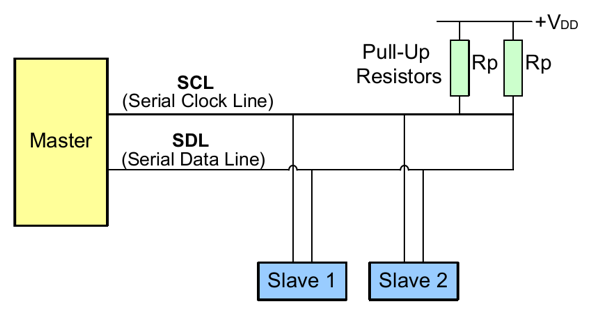
\includegraphics[width=0.7\linewidth]{ImagenesIngenieria de Detalle/I2C_conexionado}	
	\caption{Conexionado $I^2C$ Multi-slave.}
	\label{fig:conexionado_i2c}
\end{figure}


